\documentclass{beamer}
\mode<presentation>
\usepackage{amsmath}
\usepackage{amssymb}
\usepackage{bm}
\usepackage{adjustbox}
\usepackage{subcaption}
\usepackage{enumerate}
\usepackage{multicol}
\usepackage{mathtools}
\usepackage{listings}
\usepackage{url}
\def\UrlBreaks{\do\/\do-}
\usetheme{Boadilla}
\usecolortheme{lily}
\setbeamertemplate{footline}
{
  \leavevmode%
  \hbox{%
  \begin{beamercolorbox}[wd=\paperwidth,ht=2.25ex,dp=1ex,right]{author in head/foot}%
    \insertframenumber{} / \inserttotalframenumber\hspace*{2ex} 
  \end{beamercolorbox}}%
  \vskip0pt%
}
\setbeamertemplate{navigation symbols}{}

\providecommand{\nCr}[2]{\,^{#1}C_{#2}}
\providecommand{\nPr}[2]{\,^{#1}P_{#2}}
\providecommand{\mbf}{\mathbf}
\providecommand{\pr}[1]{\ensuremath{\Pr\left(#1\right)}}
\providecommand{\qfunc}[1]{\ensuremath{Q\left(#1\right)}}
\providecommand{\sbrak}[1]{\ensuremath{{}\left[#1\right]}}
\providecommand{\lsbrak}[1]{\ensuremath{{}\left[#1\right.}}
\providecommand{\rsbrak}[1]{\ensuremath{{}\left.#1\right]}}
\providecommand{\brak}[1]{\ensuremath{\left(#1\right)}}
\providecommand{\lbrak}[1]{\ensuremath{\left(#1\right.}}
\providecommand{\rbrak}[1]{\ensuremath{\left.#1\right)}}
\providecommand{\cbrak}[1]{\ensuremath{\left\{#1\right\}}}
\providecommand{\lcbrak}[1]{\ensuremath{\left\{#1\right.}}
\providecommand{\rcbrak}[1]{\ensuremath{\left.#1\right\}}}
\providecommand{\rank}{\text{rank}}
\theoremstyle{remark}
\newtheorem{rem}{Remark}
\newcommand{\sgn}{\mathop{\mathrm{sgn}}}
\providecommand{\abs}[1]{\ensuremath{\left\vert #1 \right\vert}}
\providecommand{\res}[1]{\Res\displaylimits_{#1}} 
\providecommand{\norm}[1]{\lVert#1\rVert}
\providecommand{\mtx}[1]{\mathbf{#1}}
\providecommand{\mean}[1]{\overline{#1}}
\providecommand{\fourier}{\overset{\mathcal{F}}{ \rightleftharpoons}}
\providecommand{\system}{\overset{\mathcal{H}}{ \longleftrightarrow}}
\providecommand{\dec}[2]{\ensuremath{\overset{#1}{\underset{#2}{\gtrless}}}}
\newcommand{\myvec}[1]{\ensuremath{\begin{pmatrix}#1\end{pmatrix}}}
\newenvironment{amatrix}[1]{%
  \left(\begin{array}{@{}*{#1}{c}|c@{}}
}{%
  \end{array}\right)
}
\let\vec\mathbf

\lstset{
frame=single, 
breaklines=true,
columns=fullflexible
}
\usepackage{listings}
\lstset{
  language=Python,
  basicstyle=\ttfamily\small,
  numbers=left,
  numberstyle=\tiny,
  breaklines=true,
  frame=single
}

\title{Matgeo-2.6.30}
\author{AI25BTECH11019-Menavath Sai Sanjana}

\date{}

\begin{document}

\begin{frame}
\titlepage
\end{frame}

\begin{frame}
\frametitle{Question}
If the area of a triangle is $35$ square units with vertices $(2,6)$, $(5,-4)$ and $(k,4)$, then find $k$.
\end{frame}

\begin{frame}
\frametitle{Solution}
\begin{align}
\overrightarrow{A} &= \myvec{2\\6}, \quad 
\overrightarrow{B} = \myvec{5\\-4}, \quad
\overrightarrow{C} = \myvec{k\\4}
\end{align}

\begin{align}
\overrightarrow{B}-\overrightarrow{A} &= \myvec{3\\-10}, \qquad
\overrightarrow{C}-\overrightarrow{A} = \myvec{k-2\\-2}
\end{align}
     
$
\text{Area}=\frac{1}{2}\left|\bigl(\overrightarrow{B}-\overrightarrow{A}\bigr)\times\bigl(\overrightarrow{C}-\overrightarrow{A}\bigr)\right|
$

$
35=\frac{1}{2}\left|\myvec{3\\-10}\times\myvec{k-2\\-2}\right|
$
\end{frame}

\begin{frame}
\frametitle{Solution (Continuation)}
\begin{align}
35 &=\frac{1}{2}\left|3(-2)-(-10)(k-2)\right| \\
&=\frac{1}{2}\left|-6+10k-20\right| \\
&=\frac{1}{2}\left|10k-26\right|
\end{align}

Thus,
$
|10k-26|=70
$

\begin{align}
10k-26&=70 &\Rightarrow k=\frac{48}{5} \\
10k-26&=-70 &\Rightarrow k=-\frac{22}{5}
\end{align}
\end{frame}

\begin{frame}
\frametitle{Conclusion}
\noindent\textbf{Conclusion:}  
The possible values of $k$ are
$
k=\frac{48}{5}\quad\text{or}\quad k=-\frac{22}{5}.
$
\end{frame}

\begin{frame}
\frametitle{Graphical Representation}
\begin{figure}[ht!]
    \centering
    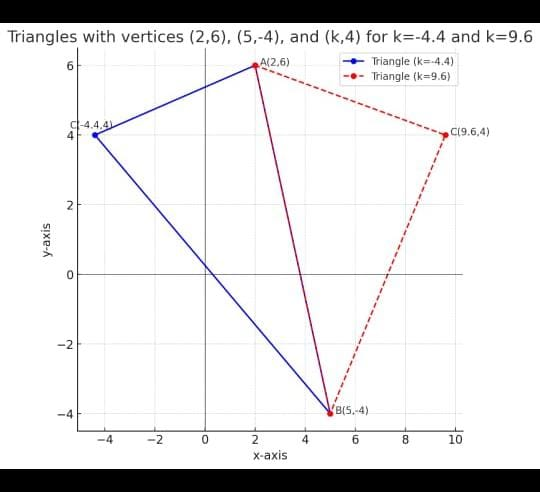
\includegraphics[width=0.65\textwidth]{matgeo-2.6.30.jpeg}
    \caption{}
    \label{fig:2.6.30}
\end{figure}
\end{frame}

\end{document}
